\chapter{TELEMAC-MASCARET \soft{Git} workflow}

In conclusion of this document, the TELEMAC-MASCARET \soft{Git} development
workflow is presented.

\begin{itemize}

\item First make sure all your shared branches are up-to-date with origin:
\begin{lstlisting}
$ git pull --rebase
\end{lstlisting}

\item Create a new local branch and start working on it (make one branch for
each new feature you plan to introduce in the code):
\begin{lstlisting}
$ git checkout -b my_branch
\end{lstlisting}

\item Push your branch to the server:
\begin{lstlisting}
$ git push --set-upstream origin my_branch
\end{lstlisting}

\item Often commit, making small commits containing specific change at a time:
\begin{lstlisting}
$ git add modified_file_1.ext folder/modified_file_2.ext
$ git commit -m "My commit message"
\end{lstlisting}
\important{Note}: use \important{git add -p} if necessary.\\

\important{Before committing, ensure that you have documented all your
changes and that you respect TELEMAC-MASCARET coding conventions.}\\

\important{All the commits must compile for debugging purposes.}

\item Once your developments are finished, you need to merge your branch with
\important{main}. First, backup your branch:
\begin{lstlisting}
$ git branch my_branch_backup
\end{lstlisting}

\item Clean up your branch using an interactive rebase on the necessary amount
of commits (\textit{e.g.} 10):
\begin{lstlisting}
$ git rebase -i HEAD~10
\end{lstlisting}
Follow the text editor instructions to clean your branch history as needed. The
idea is that \important{the history should be kept as clean as possible, so
that it is easily understood by other developers}.

\item Once you have finished cleaning the branch history, create a Merge
Request (MR) by entering the following URL on your web browser:\\
\begin{small}
\url{https://gitlab.pam-retd.fr/otm/test-telemac/-/merge_requests/new?merge_request%5Bsource_branch%5D=my_branch}
\end{small}\\
From the web page, enter a title, describe precisely what your branch does and
create the MR, as in fig.~\ref{fig:mr-creation}.

\begin{figure}[H]
  \centering
  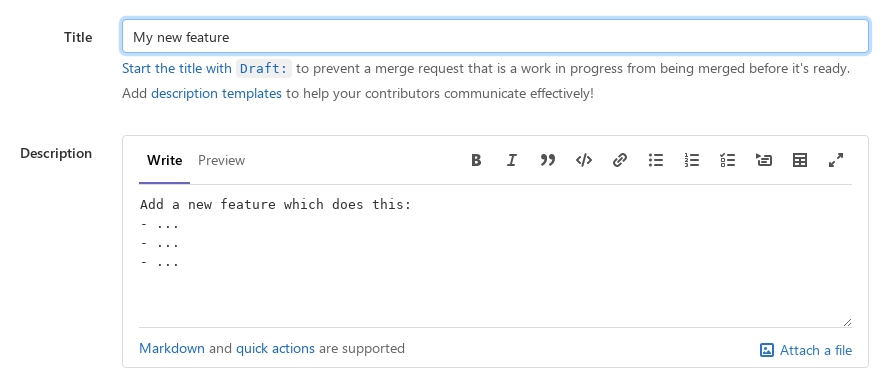
\includegraphics[scale=0.4]{graphics/mr_creation.png}
  \caption{Creation of a Merge Request}
  \label{fig:mr-creation}
\end{figure}

\item If your branch cannot be merged, \soft{GitLab} will disable the
\important{Merge} button and tell you that there are conflicts, as shown in
fig.~\ref{fig:mr-conflicts}.

\begin{figure}[H]
  \centering
  
\includegraphics[scale=0.4]{graphics/mr_conflicts.png}
  \caption{Conflicts in a Merge Request}
  \label{fig:mr-conflicts}
\end{figure}

To fix those conflicts, rebase \important{my\_branch} on top of
\important{main}:
\begin{lstlisting}
$ git rebase main
\end{lstlisting}

\item Solve each conflict \soft{Git} encountered during the rebase and
\important{make sure that the code compiles before continuing the rebase}.

\item Once the rebase is finished and that \important{you have verified that
the test-cases run correctly}, force push your branch to update your
\important{MR}:
\begin{lstlisting}
$ git push --force-with-lease
\end{lstlisting}

\important{Important}: you should never use the \important{\texttt{-{}-}force/-f} option
as other developers may have pushed new commits to the branch while you were
rebasing it. Using \important{\texttt{-{}-}force-with-lease} will prevent the update of
a branch in such a case.

\item After conflicts have been solved or if there wasn't any, the
\important{MR} can be accepted. If you have \important{Maintainer} rights on
\soft{GitLab}, you can merge it yourself. However, if the changes brought by
the \important{MR} are quite important, you should ask another developer to
review your changes, a task which can be done from the \important{MR} itself.\\

If you don't have \important{Maintainer} rights, you will need to ask for a
\important{Maintainer} to review your code changes. Maintainers can be found
from the \important{Project members} list which is available from the GitLab
project webpage.\\

\item After the \important{MR} has been accepted, delete your branch if needed
and also delete your backup branch:
\begin{lstlisting}
$ git branch -d my_branch
$ git push origin --delete my_branch
$ git branch -d my_branch_backup
\end{lstlisting}
\end{itemize}